\section{Struktur}
Softwarens struktur er bygget op omkring to sensorer som måler temperatursvingninger mellem rummet og vandrøret. I dette afsnit vil de enkelte funktionerne i softwaren til fase 1 og 2 blive beskrevet. 
\begin{figure}[h!]
  \centering
  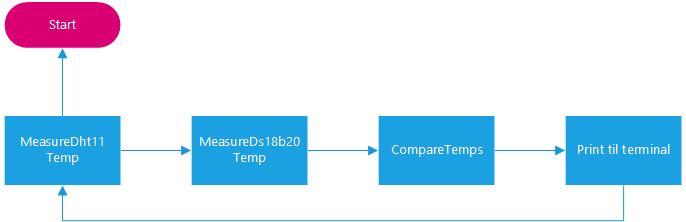
\includegraphics[width=0.5\textwidth]{figures/Fase1software2.png}
  \caption{Fase 1 - Software flowchart.}
\end{figure}


\subsection{MeasureDs18b20Temp}
\fxnote{skriv afsnit om hvordan rumtemperaturen bliver målt}

\subsection{MeasureDht11Temp}
\fxnote{skriv afsnit om hvordan rørtemperaturen bliver målt}
\subsection{CompareTemps}
\fxnote{skriv afsnit om hvordan vi sammenligner temperaturerne, og hvorfor det er brugbart}
\subsection{Print til terminal}
\fxnote{skriv afsnit om hvordan data skal vises i terminalen, muligvis andre metoder?(gem i tekstfil, smid ind i mathcad for at få graf)}

\subsection{Udvidet diagram}
\fxnote{søg på fase / phase / face i rapport og fjern så hvidt muligt, skriv som om vi udvider på rapport}
\begin{figure}[h!]
  \centering
  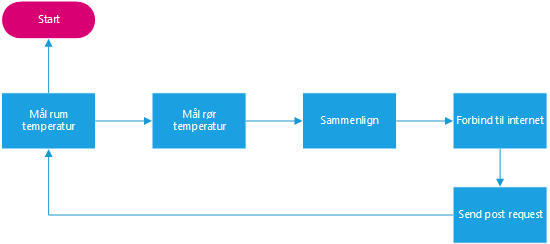
\includegraphics[width=1\textwidth]{figures/Fase2software.png}
  \caption{Fase 2 - Software flowchart.\fxnote{farv nye ting rød på figur}}
\end{figure}